\documentclass[10pt]{article}
\usepackage[polish]{babel}
\usepackage[utf8]{inputenc}
\usepackage[T1]{fontenc}
\usepackage{amsmath}
\usepackage{amsfonts}
\usepackage{amssymb}
\usepackage[version=4]{mhchem}
\usepackage{stmaryrd}
\usepackage{graphicx}
\usepackage[export]{adjustbox}
\graphicspath{ {./images/} }

\title{LIGA MATEMATYCZNA \\
 PÓŁFINAE 5 lutego 2010 \\
 SZKOŁA PODSTAWOWA }

\author{}
\date{}


\begin{document}
\maketitle
\section*{ZADANIE 1.}
Arbuz jest o \(\frac{4}{5} \mathrm{~kg}\) cięższy od \(\frac{4}{5}\) tego arbuza. Ile waży arbuz?

\section*{ZADANIE 2.}
W pewnej rodzinie jest czworo dzieci w wieku 5, 8, 13 i 15 lat. Imiona tych dzieci to Ania, Bartek, Czesia i Daria. Ile lat ma każde z nich, jeżeli jedna dziewczynka chodzi do przedszkola, Ania jest starsza od Bartka, a suma lat Ani i Czesi dzieli się przez 3?

\section*{ZADANIE 3.}
Do hurtowni nadszedł transport trzech gatunków herbaty. Każdego gatunku było tyle samo, a cały transport ważył mniej niż 4 tony. Pierwszy gatunek herbaty przysłano w 76 jednakowych paczkach, drugi w 57 jednakowych paczkach, a trzeci w 60 jednakowych paczkach. W każdej paczce była całkowita liczba kilogramów herbaty. Ile nadeszło herbaty każdego gatunku? Ile herbaty było w każdej z trzech rodzajów paczek?

\section*{ZADANIE 4.}
Tablicę \(3 \times 3\) podzielono na dziewięć jednakowych kwadratów. W każdy z nich wpisano liczbę -1 lub 0, lub 1. Wykaż, że wśród wszystkich sum z trzech wierszy, trzech kolumn i dwóch głównych przekątnych co najmniej dwie są równe.

\section*{ZADANIE 5.}
Cztery kwadratowe płytki ułożono jak na rysunku. Długości boków dwóch z tych płytek zaznaczono na rysunku. Jaka jest długość boku największej płytki?\\
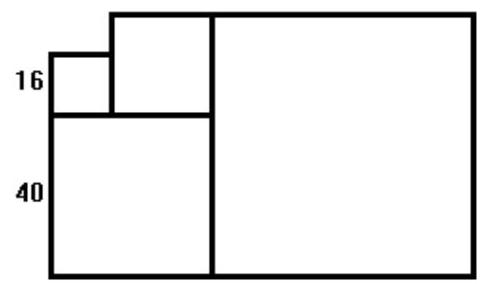
\includegraphics[max width=\textwidth, center]{2024_11_21_d884d372f0f6df0e5406g-1}


\end{document}